\documentclass[tikz,border=3pt]{standalone}
\usetikzlibrary{positioning,arrows.meta,shapes.geometric,backgrounds}

\begin{document}
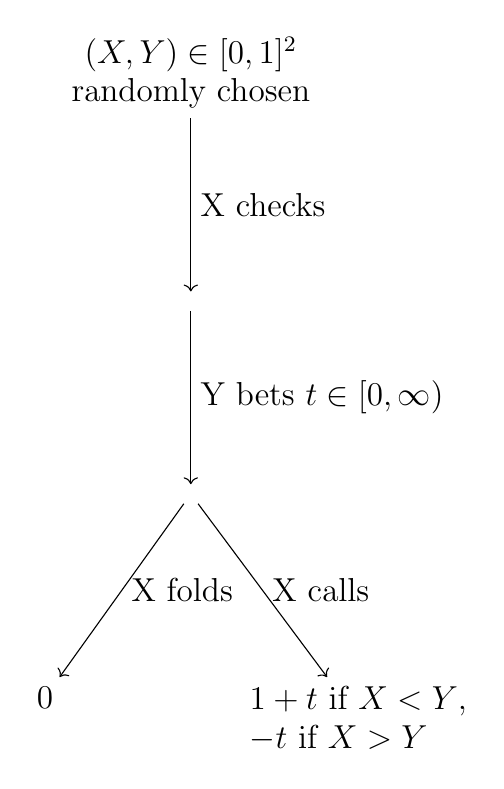
\begin{tikzpicture}

% nodes (manual positions for clearer layout)
\node[align=center, font=\large] (root) {$(X,Y)\in[0,1]^2$ \\randomly chosen};
\node[below=22mm of root] (xcheck) {};
\node[align=center, below =22mm of xcheck] (ybet) {};
\node[below left=22mm and 15mm of ybet, font=\large] (xfold) {$0$};
\node[below right=22mm and 5mm of ybet, font=\large, align=left] (xcall) {
$1 + t$ if $X < Y$, \\
$-t$ if $X > Y$
};

% edges with labels
\draw[->] (root) -- (xcheck) node[midway,right, font=\large] {X checks};
\draw[->] (xcheck) -- (ybet) node[midway,right, font=\large] {Y bets $t \in [0,\infty)$};

\draw[->] (ybet) -- (xfold) node[midway,right, font=\large] {X folds};
\draw[->] (ybet) -- (xcall) node[midway,right, font=\large] {X calls};

\end{tikzpicture}
\end{document}
